\renewcommand{\nomebreve}{is\_shuffle\_of}
\renewcommand{\titolo}{Can a deck of cards be obtained as the shuffle of two?}

\introduzione{}

Scusate i due titoli (breve e lungo)
entrambi in inglese, ma non sapevo come rendere il concetto di \emph{shuffle} in italiano e l'indicizzabilità trasparente dei problemi che stiamo accumulando resta un valore, inclusa l'immediatezza del titolo.
In inglese credo che basti una parola per rendere l'idea mentre in italiano vediamo se mi riesce di spiegarmi (dove resta oscuro voi all'esame chiedete, ok? Non è sui linguaggi e formalismi che intendiamo misurarci all'esame di algo):\\

\noindent
  \begin{minipage}[c]{.48\textwidth}
     \emph{\bf shuffle:}\/ partendo da due mazzi di carte, l'operazione di shuffle compone un unico mazzo inframmezzando le carte dei due in un unico ordine. Di solito viene eseguita ponendo i due mazzi a faccia in giù sul tavolo verde, avvicinando due angoli dei mazzi fino a toccarsi ed aderendovi coi pollici, scorrendo quindi i pollici verso l'alto (come a far frusciare dollaroni) facendo in modo che le carte dei due mazzi, ricadendo in basso, si inframmezzino a pettine.
   \end{minipage}%
\hspace{8.0mm}%
\begin{minipage}[c]{.50\textwidth}
   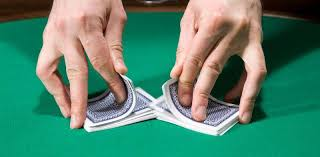
\includegraphics[scale=0.7]{figs/card_shuffle.jpeg}
\end{minipage}

\medskip

  \begin{minipage}[c]{.40\textwidth}
    Ad esempio, partendo dai due mazzi:
    \begin{description}
      \item[{\sc Mazzo~$x$:}] 7, 2, K
      \vspace{-2mm}
      \item[{\sc Mazzo~$y$:}] K, 7, 2, 7
    \end{description}
  \end{minipage}%
\hspace{8.0mm}%
  \begin{minipage}[c]{.50\textwidth} 
    Alcuni possibili shuffle di $x$ ed $x$ sono:\\
    \indent 7, 2, K, K, 7, 2, 7 (semplice concatenazione)\\
    \indent 7, 2, K, 7, K, 2, 7 (unico shuffle palindromo?)\\
    \indent 7, 2, K, 7, 2, K, 7 (anche il 2 scavalca il K)\\
  \end{minipage}

... ohi, ohi, le possibilità andranno a crescere in modo esponenziale,
ma ora provo a formalizzare il concetto:

data una sequenza $x$ (il primo mazzo)
di $m$ numeri naturali $x_1, \ldots, x_m$
ed una sequenza $y$ (il secondo mazzo)
di $n$ numeri naturali $y_1, \ldots, y_n$,
ed una sequenza binaria $b$ di $m+n$ bits di non-determinismo,
potremmo definire \emph{lo shuffle di $x$ ed $y$ dettato da $b$}
come quella stringa $w$ di lunghezza $m+n$ tale che

\[
w[i] = \left\{
         \begin{array}{ll}
          x[i- num\_ones(b_i)] & \mbox{ if $b[i]=0$} \\
          y[i- num\_zeros(b_i)] & \mbox{ if $b[i]=1$}
         \end{array}
       \right.
\]

dove abbiamo indicato con $b_i$ il prefisso di $b$ di lunghezza~$i$,
mentre le funzioni $num\_ones(\cdot)$ e $num\_zeros(\cdot)$
ritornano, rispettivamente, il numero di uni e di zeri entro la stringa binaria presa ad argomento.\\

\noindent
Definito cosa sia lo shuffle in italiano, eccovi il problema:

\begin{quote}
  il crupier doveva fare lo shuffle di due mazzi a me noti, $x$ ed $y$, e dice di aver prodotto un mazzo $w$. Dice la verità o è un baro?
  
  E se dice la verità, sapresti offrire una spiegazione di come sia potuto succedere specificando
  una stringa binaria $b$ tale che $w$ sia lo shuffle di $x$ ed $y$ dettato da $b$?
\end{quote}

\sezionetesto{Dati di input}
La prima riga del file \verb'input.txt' contiene i numeri interi e positivi $m$, $n$ e $t$, nell'ordine, dove $t\in \{0,1\}$ specifica meglio il tipo di output desiderato.
La seconda (o terza, o quarta) riga contiene $m$ (o $n$, o $m+n$; rispettivamente) numeri naturali l'$i$-esimo dei quali è $x[i]$ (o $y[i]$, o $w[i]$; rispettivamente).
Ovviamente, quando su una stessa riga, tutti i numeri di cui parliamo sono separati da spazi.

\sezionetesto{Dati di output}
Nella prima riga del file \verb'output.txt' si scriva un unico numero:
$1$ se $w$ può essere ottenuto come shuffle di $x$ e di $y$, altrimenti $0$.

Se $t=0$ il file non deve contenere ulteriori righe.
Se $t=1$ ed il numero scritto nella prima riga del file \verb'output.txt'
è anche esso un $1$, allora, nella seconda ed ultima riga del file \verb'output.txt' si riportino, separati da spazi, gli $m+n$ bits della sequenza $b$
lessicograficamente minima tale che
$w$ è lo shuffle di $x$ ed $y$ dettato da $b$.\\


% Esempi
\sezionetesto{Esempio di input/output}
\esempio{
3 4 0

7 2 13

13 7 2 7

13 7 7 2 2 7 13
}{1}

\esempio{
3 4 1

7 2 13

13 7 2 7

13 7 2 7 2 7 13
}{1

1 0 0 1 1 1 0}

\esempio{
3 4 1

7 2 13

13 7 2 7

13 7 7 7 2 2 13
}{0}

\section*{Assunzioni}

$m,n \leq 1000$, i numeri nelle sequenze sono interi nell'intervallo $[0,10\,000]$.

\section*{Subtask}

  \begin{itemize}
    \item \textbf{Subtask 1 [0 punti]:} i tre esempi del testo.
    \item \textbf{Subtask 2 [20 punti]:} $m+n \leq 20$, tipo~$0$.
    \item \textbf{Subtask 3 [10 punti]:} $m+n \leq 20$, tipo~$1$.
    \item \textbf{Subtask 4 [20 punti]:} $x=0^m$ ossia la prima sequenza contiene solo zeri, tipo~$0$.
    \item \textbf{Subtask 5 [10 punti]:} $x=0^m$ ossia la prima sequenza contiene solo zeri, tipo~$1$.
    \item \textbf{Subtask 6 [25 punti]:} $m,n \leq 1000$, tipo~$0$.
    \item \textbf{Subtask 7 [15 punti]:} $m,n \leq 1000$, tipo~$1$.      
  \end{itemize}
  
